

\section{Elastiklik kuchi}

\begin{enumerate}

\item Prujinaning bikrligi – bu elastiklik kuchining prujinaning ... ga nisbatidir.
\begin{enumerate}[label=\Alph*)]
\item vazni
\item massasi
\item diametri
\item absolyut deformatsiyasi kattaligi
\end{enumerate}

\item 3 N kuch ta’sirida prujina 6 mm ga cho‘zildi. Prujinaning bikrligini toping (N/m).
\begin{enumerate}[label=\Alph*)]
\item 2000
\item 20
\item 200
\item 500
\end{enumerate}

\item Massasi 2 kg yuk ta’sirida 4 sm ga uzaygan prujinaning bikrligini toping (N/m).
\begin{enumerate}[label=\Alph*)]
\item 2000
\item 20
\item 200
\item 500
\end{enumerate}

\item Bikrligi 200 N/m bo‘lgan prujina 10 N kuch ta’sirida qanchaga cho‘ziladi (sm)?
\begin{enumerate}[label=\Alph*)]
\item 5
\item 20
\item 0,05
\item 2
\end{enumerate}

\item Bikrligi 6 kN/m bo‘lgan prujina 900 N kuch ta’sirida qanchaga cho‘ziladi (sm)?
\begin{enumerate}[label=\Alph*)]
\item 15
\item 0,67
\item 0,15
\item 6,67
\end{enumerate}

\item 4 kg yuk osilganda 4 sm uzunlikdagi prujina 2 mm uzaygan. Prujinaning bikrligi qanday (kN/m)?
\begin{enumerate}[label=\Alph*)]
\item 0,5
\item 5
\item 50
\item 20
\end{enumerate}

\item Bikrligi 30 kN/m bo‘lgan prujinani 4 sm ga cho‘zish uchun kerak bo‘ladigan kuch necha (N)?
\begin{enumerate}[label=\Alph*)]
\item 120
\item 1200
\item 12
\item 12000
\end{enumerate}

\item 4 N kuch ta’sirida 5 sm ga uzaygan prujinaning bikrligini toping (N/m).
\begin{enumerate}[label=\Alph*)]
\item 8,9
\item 80
\item 8,7
\item 8,8
\end{enumerate}

\item Metall sterjenning absolyut va nisbiy uzayishi mos holda 2 mm va 0,1 foiz bo‘lsa, deformatsiyalanmagan sterjenning uzunligi qanday (m)?
\begin{enumerate}[label=\Alph*)]
\item 0,2
\item 1
\item 2
\item 4
\end{enumerate}

\item 1 t massali avtomobilni $1 m/s^2$ tezlanish bilan shatakka olishda bikrligi 100 kN/m bo‘lgan tros qanchaga (sm) cho‘ziladi? Ishqalanishni hisobga olmang.
\begin{enumerate}[label=\Alph*)]
\item 4
\item 1
\item 3
\item 2
\end{enumerate}

\item Dinamometr prujinasi 4 N kuch ta’sirida 5 mm cho‘zildi. Prujinani 16 mm cho‘zadigan yukning og‘irligini aniqlang (N).
\begin{enumerate}[label=\Alph*)]
\item 12,8
\item 42,4
\item 1,28
\item 8,12
\end{enumerate}

\item Rezina shnurga osib qo‘yilgan 4,9 N og‘irlikdagi yuk yuqoriga $2 m/s^2$ tezlanish bilan ko‘tarilayotgan bo‘lsa, rezina shnurning uzayishini (m) toping. Rezina bikrligi 980 N/m ga teng.
\begin{enumerate}[label=\Alph*)]
\item $6 \cdot 10^{-2}$
\item $6 \cdot 10^{-3}$
\item 0,6
\item $5 \cdot 10^{-3}$
\end{enumerate}

\item Grafiklarning qaysi biri Guk qonunini to‘g‘ri tavsiflaydi?

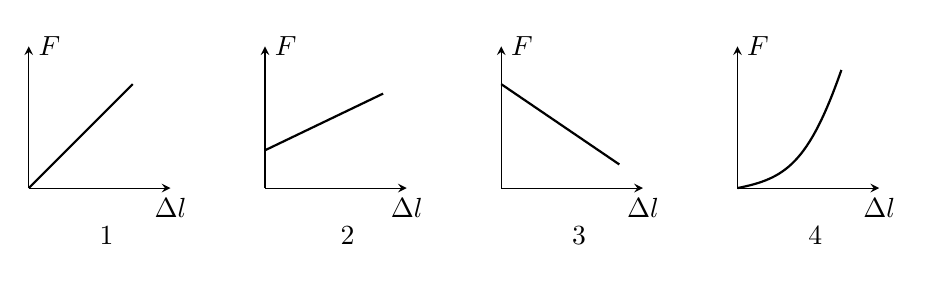
\begin{tikzpicture}[>=stealth, scale=0.6]
    % --- 1-grafik (To'g'ri javob: To'g'ri proporsional) ---
    \begin{scope}[xshift=0cm, yshift=4cm]
        \draw[->] (0,0) -- (3,0) node[below] {$\Delta l$};
        \draw[->] (0,0) -- (0,3) node[right] {$F$};
        \draw[thick] (0,0) -- (2.2,2.2);
        \node[left] at (2,-1) {1};
    \end{scope}

    % --- 2-grafik (Boshlang'ich kuch bilan) ---
    \begin{scope}[xshift=5cm, yshift=4cm]
        \draw[->] (0,0) -- (3,0) node[below] {$\Delta l$};
        \draw[->] (0,0) -- (0,3) node[right] {$F$};
        \draw[thick] (0,0.8) -- (2.5,2);
        \node[left] at (2.1,-1) {2};
    \end{scope}

    % --- 3-grafik (Teskari bog'lanish) ---
    \begin{scope}[xshift=10cm, yshift=4cm]
        \draw[->] (0,0) -- (3,0) node[below] {$\Delta l$};
        \draw[->] (0,0) -- (0,3) node[right] {$F$};
        \draw[thick] (0,2.2) -- (2.5,0.5);
        \node[left] at (2,-1) {3};
    \end{scope}

    % --- 4-grafik (Egri chiziqli bog'lanish) ---
    \begin{scope}[xshift=15cm, yshift=4cm]
        \draw[->] (0,0) -- (3,0) node[below] {$\Delta l$};
        \draw[->] (0,0) -- (0,3) node[right] {$F$};
        \draw[thick] (0,0) .. controls (1,0.2) and (1.5,0.5) .. (2.2,2.5);
        \node[left] at (2,-1) {4};
    \end{scope}
\end{tikzpicture}

\begin{enumerate}[label=\Alph*)]
\item 1
\item 2
\item 3
\item 4
\end{enumerate}

\item Prujina uzunligi o‘zgarishining unga qo‘yilgan kuchga bog‘lanish grafigi rasmda keltirilgan. Prujinaning bikrligini aniqlang (N/m).

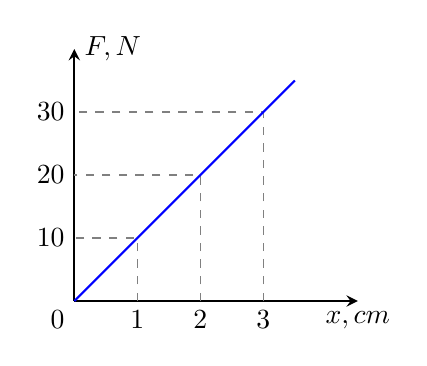
\begin{tikzpicture}[>=stealth, scale=0.8]
    % Koordinata o'qlari
    \draw[->, thick] (0,0) -- (4.5,0) node[below] {$x, cm$};
    \draw[->, thick] (0,0) -- (0,4) node[right] {$F, N$};

    % Yordamchi punktir chiziqlar (proyeksiyalar)
    \draw[dashed, gray] (1,0) -- (1,1) -- (0,1);
    \draw[dashed, gray] (2,0) -- (2,2) -- (0,2);
    \draw[dashed, gray] (3,0) -- (3,3) -- (0,3);

    % Grafik chizig'i
    \draw[thick, blue] (0,0) -- (3.5,3.5);

    % O'qlardagi qiymatlar
    \node[below left] at (0,0) {0};
    \node[below] at (1,0) {1};
    \node[below] at (2,0) {2};
    \node[below] at (3,0) {3};
    
    \node[left] at (0,1) {10};
    \node[left] at (0,2) {20};
    \node[left] at (0,3) {30};

\end{tikzpicture}

\begin{enumerate}[label=\Alph*)]
\item 10
\item 500
\item 1000
\item 90
\end{enumerate}

\item Elastiklik kuchining proeksiyasi qanday ifoda bilan aniqlanadi?
\begin{enumerate}[label=\Alph*)]
\item $-k\Delta l$
\item $k\Delta l$
\item $k/\Delta l$
\item $\Delta l/l_0$
\end{enumerate}

\item Rasmda keltirilgan grafik bo‘yicha prujinaning bikrligini aniqlang.

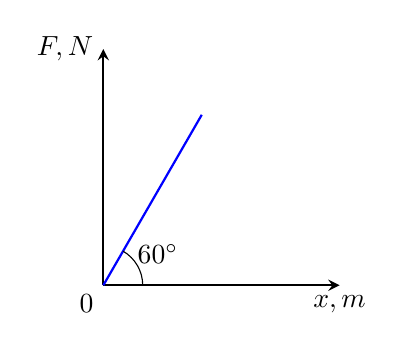
\begin{tikzpicture}[>=stealth, scale=1]
    % Koordinata o'qlari
    \draw[->, thick] (0,0) -- (3,0) node[below] {$x, m$};
    \draw[->, thick] (0,0) -- (0,3) node[left] {$F, N$};

    % Grafik chizig'i (60 gradus burchak ostida)
    % Uzunligi ixtiyoriy 2.5 birlik qilib olindi
    \draw[thick, blue] (0,0) -- (60:2.5);

    % Burchakni ko'rsatish (yoy)
    \draw (0.5,0) arc (0:60:0.5);
    \node at (30:0.8) {$60^\circ$};

    % Boshlang'ich nuqta
    \node[below left] at (0,0) {0};

\end{tikzpicture}

\begin{enumerate}[label=\Alph*)]
\item $\sqrt{3}/3$
\item $\sqrt{3}/2$
\item 1
\item $\sqrt{3}$
\end{enumerate}

\item A Devordan rasmda ko‘rsatilgandek oshib o‘tish uchun mutlaq elastik P prujina ustiga o‘rnatilgan supachaga M minoraning kamida qaysi pog‘onasidan sakrash kerak bo‘ladi?

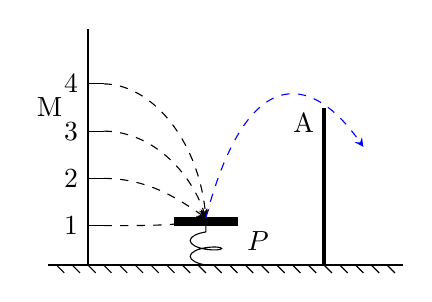
\begin{tikzpicture}[>=stealth, scale=1]
    % Yer (ground)
    \draw[thick] (-0.5,0) -- (4,0);
    \foreach \x in {-0.4,-0.2,0,0.2,0.4,0.6,0.8,1.0,1.2,1.4,1.6,1.8,2.0,2.2,2.4,2.6,2.8,3.0,3.2,3.4,3.6,3.8}
        \draw (\x,0) -- (\x+0.1,-0.1);

    % M Minora (chapda)
    \draw[thick] (0,0) -- (0,3);
    \node[left] at (-0.2,2) {M};
    
    % Minoradagi pog'onalar (1, 2, 3, 4)
    \foreach \y/\n in {0.5/1, 1.1/2, 1.7/3, 2.3/4} {
        \draw (0,\y) -- (0.2,\y);
        \node[left] at (0,\y) {\n};
    }

    % P Prujina va supacha (markazda)
    \draw[decoration={aspect=0.3, segment length=2mm, amplitude=2mm, coil}, decorate] (1.5,0) -- (1.5,0.5);
    \filldraw[black] (1.1,0.5) rectangle (1.9,0.6); % Supacha
    \node[right] at (1.9,0.3) {$P$};

    % D Devor (o'ngda)
    \draw[ultra thick] (3,0) -- (3,2);
    \node[left] at (3,1.8) {A};

    % Traektoriyalar (punktir chiziqlar)
    % Minoradan supachaga
    \draw[dashed, ->] (0.2,0.5) .. controls (0.8,0.5) and (1.2,0.5) .. (1.5,0.6);
    \draw[dashed, ->] (0.2,1.1) .. controls (0.8,1.1) and (1.2,0.8) .. (1.5,0.6);
    \draw[dashed, ->] (0.2,1.7) .. controls (0.8,1.7) and (1.3,1.2) .. (1.5,0.6);
    \draw[dashed, ->] (0.2,2.3) .. controls (0.8,2.3) and (1.4,1.6) .. (1.5,0.6);

    % Supachadan devor osha (sakrash)
    \draw[dashed, ->, blue] (1.5,0.6) .. controls (2.0,2.5) and (2.8,2.5) .. (3.5,1.5);

\end{tikzpicture}

\begin{enumerate}[label=\Alph*)]
\item 1
\item 2
\item 3
\item 4
\end{enumerate}

\item Rasmda ko‘rsatilgan, bikrligi 600 N/m bo‘lgan vaznsiz prujina 2 sm ga cho‘zilishi uchun aravacha qanday ($m/s^2$) tezlanish bilan harakatlanishi kerak? (Ishqalanishni hisobga olmang, $m=5$ kg).

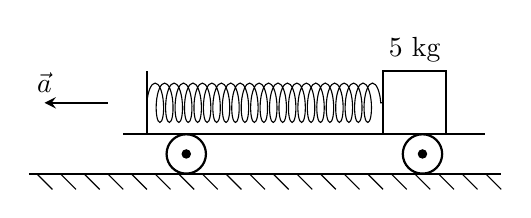
\begin{tikzpicture}[>=stealth, scale=1]
    % Yer (ground)
    \draw[thick] (-1.5,0) -- (4.5,0);
    \foreach \x in {-1.4,-1.1,...,4.3}
        \draw (\x,0) -- (\x+0.2,-0.2);

    % G'ildiraklar
    \draw[fill=white, thick] (0.5, 0.25) circle (0.25);
    \filldraw (0.5, 0.25) circle (1.5pt);
    \draw[fill=white, thick] (3.5, 0.25) circle (0.25);
    \filldraw (3.5, 0.25) circle (1.5pt);

    % Aravacha platformasi
    \draw[thick] (-0.3, 0.5) -- (4.3, 0.5);
    
    % Chap tomondagi vertikal tayanch
    \draw[thick] (0, 0.5) -- (0, 1.3);

    % Yuk (5 kg)
    \draw[thick] (3, 0.5) rectangle (3.8, 1.3);
    \node[above] at (3.4, 1.3) {5 kg};

    % Prujina
    \draw[decoration={aspect=0.3, segment length=1.2mm, amplitude=2.5mm, coil}, decorate] (0, 0.9) -- (3, 0.9);

    % Tezlanish vektori (a)
    \draw[->, thick] (-0.5, 0.9) -- (-1.3, 0.9) node[above] {$\vec{a}$};

\end{tikzpicture}

\begin{enumerate}[label=\Alph*)]
\item 15
\item 2,4
\item 0,42
\item 1,67
\end{enumerate}

\item Uzunliklari bir xil bo‘lib, bir uchlari birlashtirilgan ikkita prujinaning bo‘sh uchlaridan ushlab cho‘zamiz. Bunda bikrligi 100 N/m bo‘lgan prujina 5 sm uzayadi. Ikkinchi prujina 1 sm uzaysa, uning bikrligi qanday (kN/m)?
\begin{enumerate}[label=\Alph*)]
\item 0,5
\item 50
\item 0,25
\item 0,2
\end{enumerate}

\item Uzunligi 1 m bo‘lgan po‘lat simning uchiga massasi 260 g bo‘lgan jism biriktirilgan. Bu jism 2 ayl/s chastota bilan aylantirilganda qancha uzayadi? Simning bikrligi 5000 N/m.
\begin{enumerate}[label=\Alph*)]
\item 2,5 sm
\item 8,2 mm
\item 4 sm
\item 2,5 mm
\end{enumerate}

\end{enumerate}




\begin{table}[h!]
\centering
\caption{16-§. Elastiklik kuchi. Guk qonuni bo'yicha to'g'ri javoblar jadvali}
\begin{tabular}{|l|c|c|c|c|c|c|c|c|c|c|}
\hline
\textbf{Savol №} & 1 & 2 & 3 & 4 & 5 & 6 & 7 & 8 & 9 & 10 \\ \hline
\textbf{Javob}   & E & D & D & A & A & D & B & B & C & B \\ \hline
\hline
\textbf{Savol №} & 11 & 12 & 13 & 14 & 15 & 16 & 17 & 18 & 19 & 20 \\ \hline
\textbf{Javob}   & A & B & A & C & A & D & C & B & A & B \\ \hline
\end{tabular}
\end{table}